 \thispagestyle{gocconone}
\pagestyle{gocco}
\everymath{\color{gocco}}
\graphicspath{{../gocco/pic/}}
\blfootnote{$^1${\color[named]{gocco}Trung tâm Quy hoạch và Điều tra tài nguyên -- môi trường biển khu vực phía Nam.}}
\begingroup
\AddToShipoutPicture*{\put(0,616){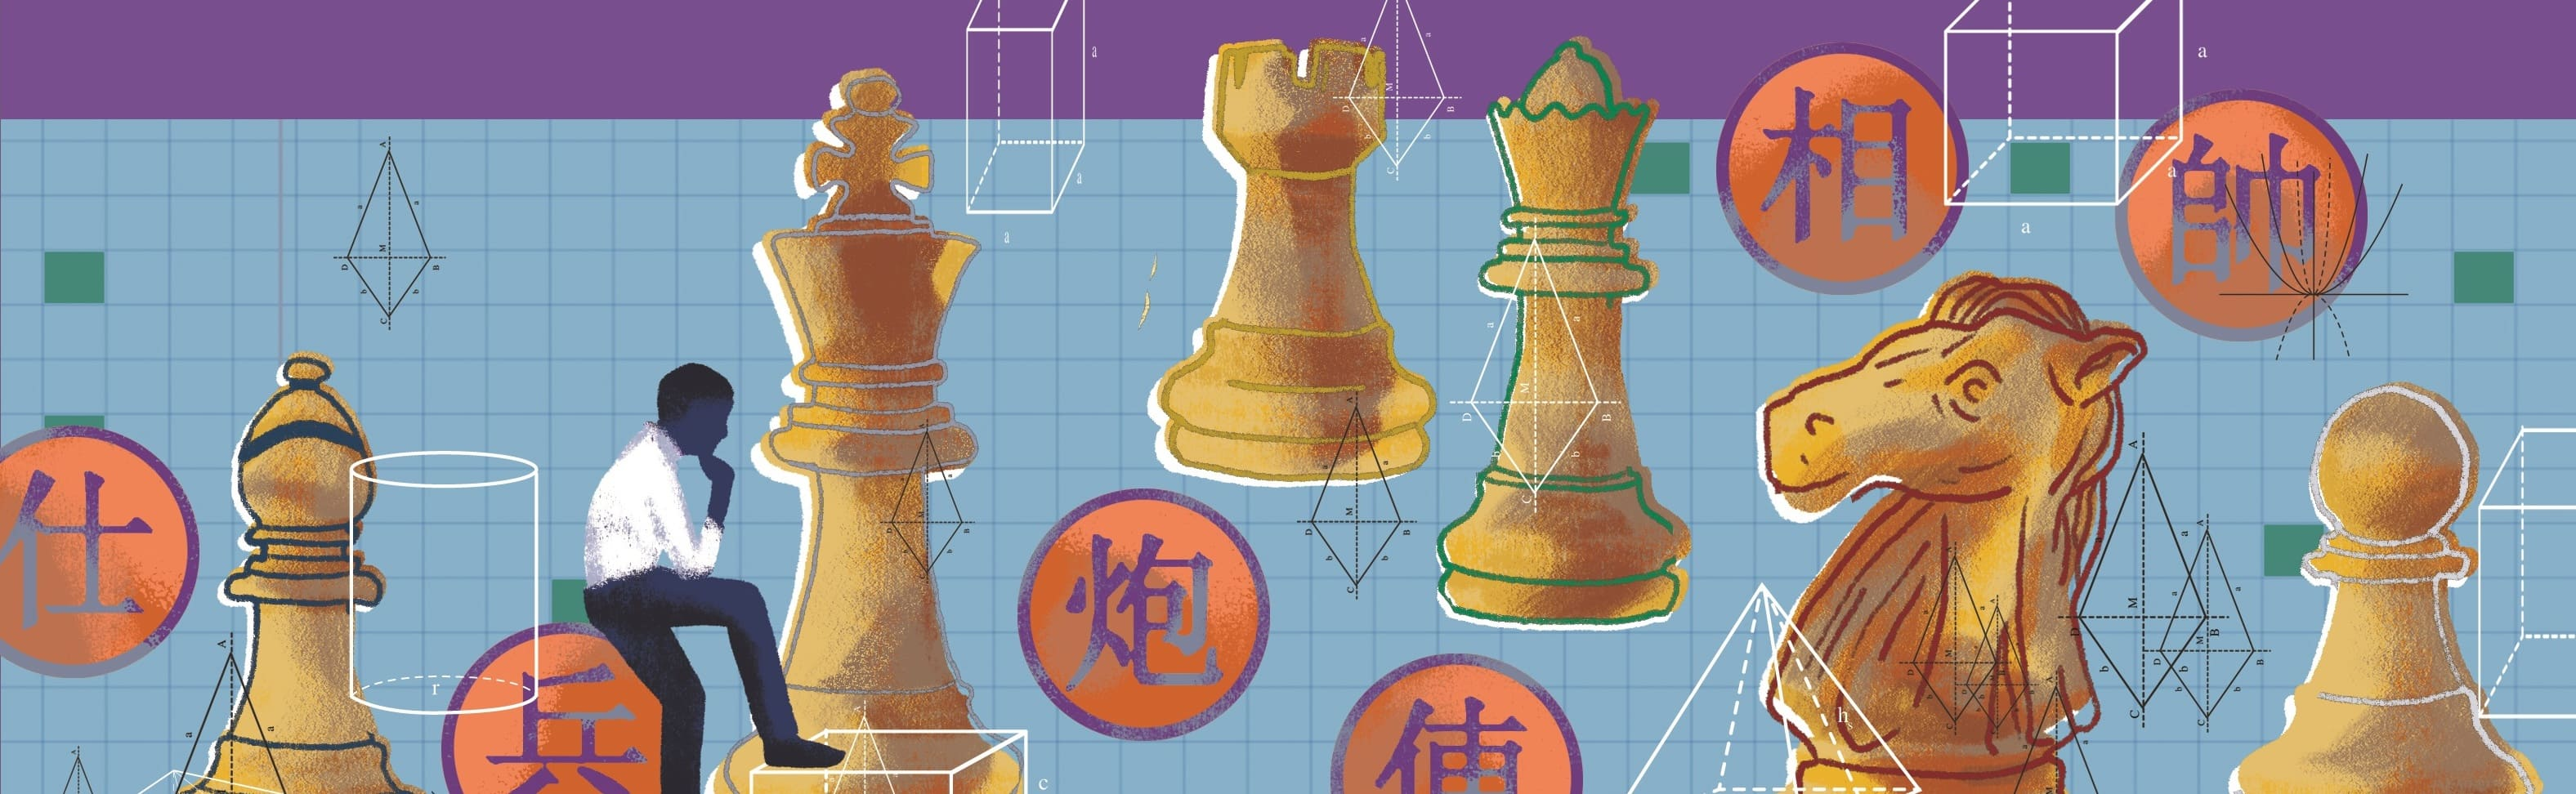
\includegraphics[width=19.3cm]{../bannergocco}}}
\AddToShipoutPicture*{\put(55,557){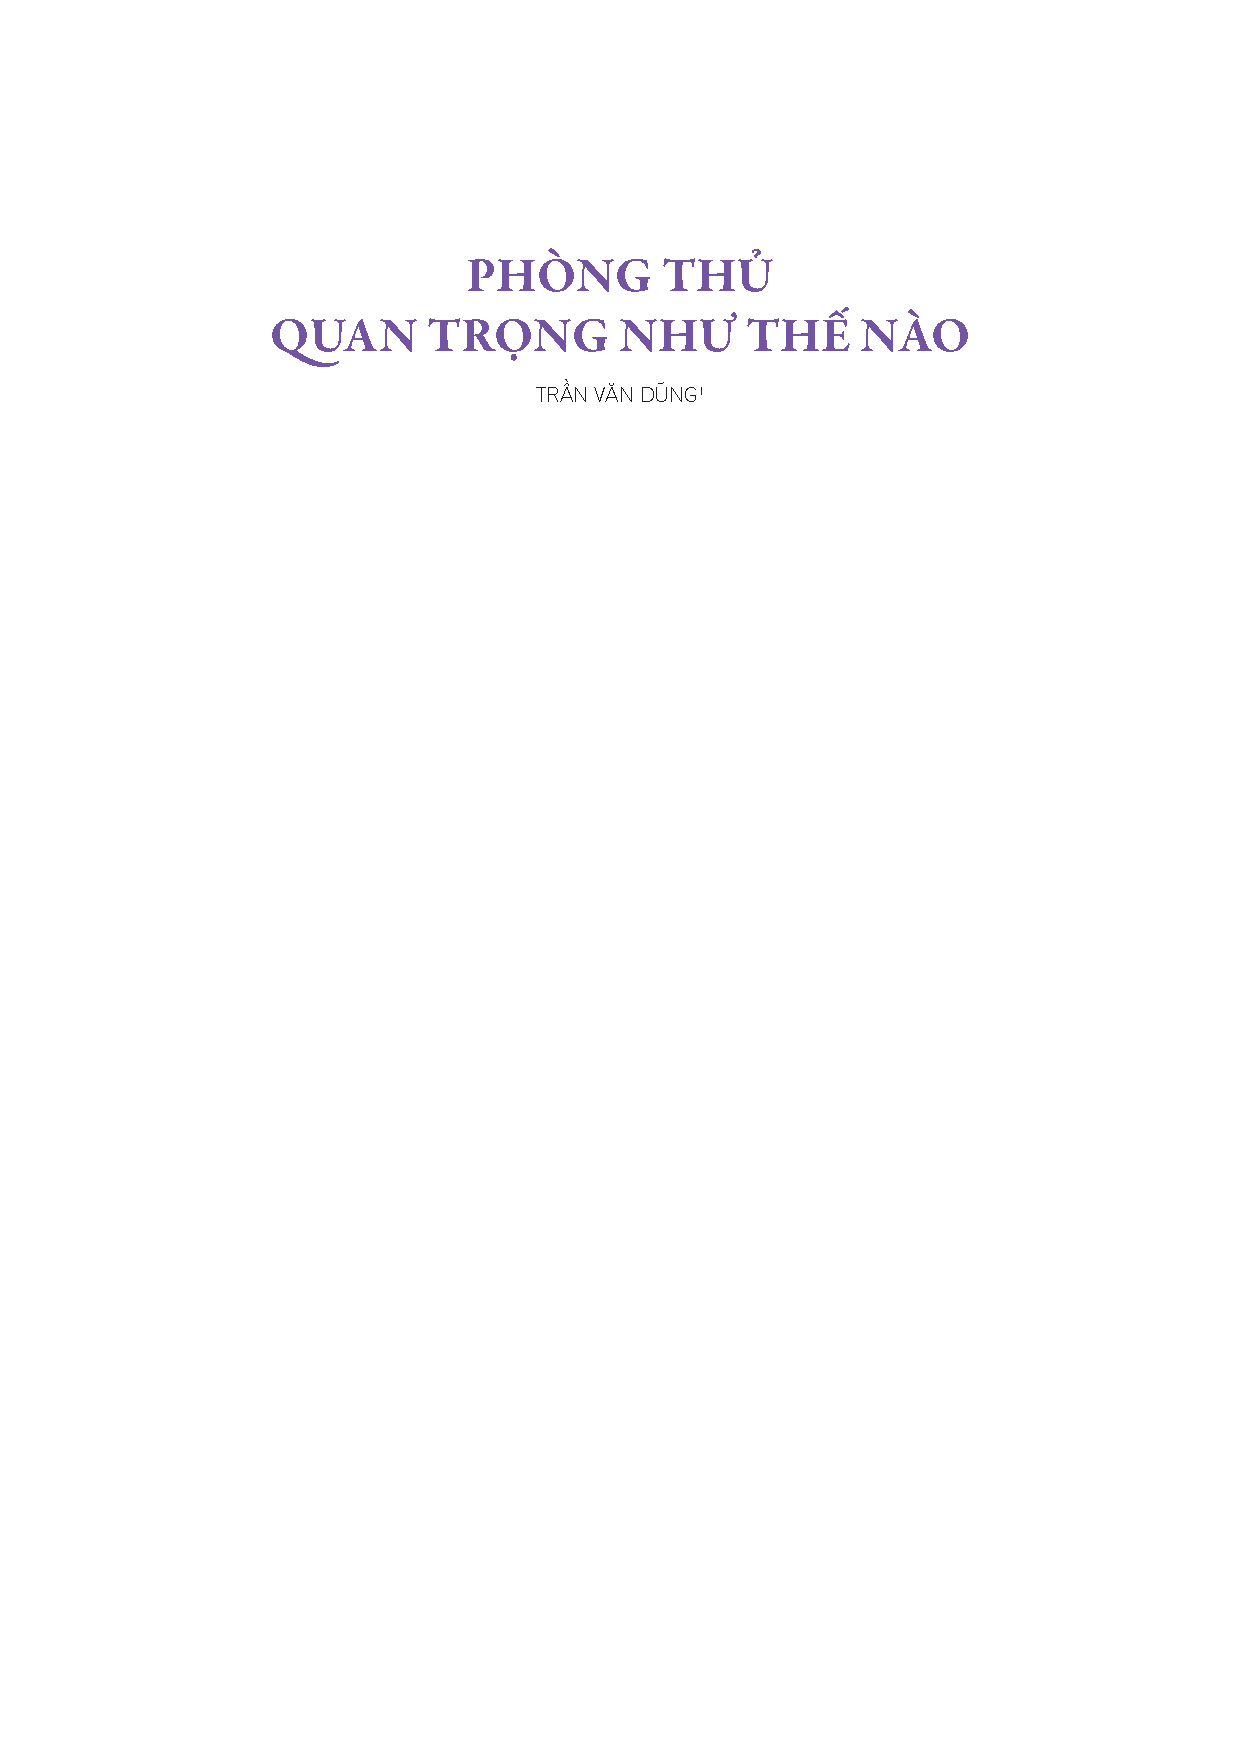
\includegraphics[scale=0.95]{../tieude2.pdf}}} 
\centering
\endgroup

\vspace*{150pt}
\begin{multicols}{2}
	Cùng với Sĩ, quân Tượng trong Cờ Tướng có tính chất phòng thủ điển hình, vai trò chủ yếu là che chắn, chống đỡ những đợt tấn công của kẻ thù để bảo đảm sự an toàn cho Tướng. Quân Tượng theo luật Cờ Tướng có một số bó buộc và hạn chế nhất định: mỗi nước chỉ được di chuyển theo đường chéo hai ô một (hình chữ Điền);  không được qua bên kia sông để tiến vào trận địa của kẻ địch. Như vậy, mỗi một quân Tượng khi vào trận  chỉ có thể lui tới bảy điểm cố định sẵn có trên bàn cờ.
	\vskip 0.05cm
	Nhưng không phải vì những điều đó mà Tượng mất đi tầm quan trọng cũng như vị thế vốn có của mình. Khi vào trận chiến, hai quân Tượng cùng nhau khéo léo phối hợp, hỗ trợ, liên kết chặt chẽ với song Sĩ để tạo ra một bức tường phòng thủ kiên cố. Những bước di chuyển của Tượng, thoạt nhìn thì có thể rất giản đơn, đôi khi còn bị coi là thừa thãi, nhưng nếu được suy xét kỹ thì có thể thấy, chúng đều có những mục đích nhất \linebreak định. Lúc bình ổn Tượng được điều lên đường số năm để làm rắn chắc trung lộ, khi cấp thiết thì sẵn sàng án ngữ trên bờ sông hay dạt ra biên để chặn đứng bước nhảy khó lường của chiến Mã đối phương. Bước sang giai đoạn tàn cuộc, với số quân lực còn lại ít ỏi, Tượng có thể được dùng để giữ mặt, tạo thêm thời gian cũng như không gian cho Tướng ẩn náu, tránh né những hướng tấn công nguy hiểm của đối phương. 
	\vskip 0.05cm
	Ngoài nhiệm vụ giữ vững hậu phương, trong nhiều tình huống Tượng còn là công cụ hỗ trợ đắc lực cho tiền tuyến, có thể trở thành điểm tựa vững chắc cho chiến Mã phục kích trên hà hoặc làm ngòi nổ cho Pháo, tạo ra những đợt phản kích bất ngờ, đánh phá cửu cung, bắt sống Tướng giặc.
	\vskip 0.05cm
	Sau đây tác giả xin đưa ra một vài ví dụ điển hình  để minh chứng cho những tác dụng, tính năng khác nhau của quân Tượng:
		\begin{figure}[H]
		\vspace*{-5pt}
		\centering
		\captionsetup{labelformat= empty, justification=centering}
		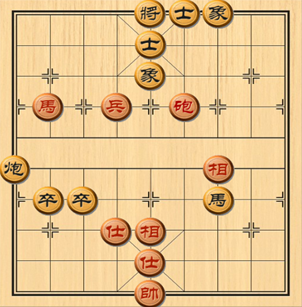
\includegraphics[width= 0.35\textwidth]{1}
		\caption{\small\textit{\color{gocco}Hình $1$.}}
		\vspace*{-10pt}
	\end{figure}
	$1.$ Hình  $1$, đây là hình cờ tàn cơ bản, nếu như bên Đen có đầy đủ bộ phòng thủ (Sĩ, Tượng), bên Đỏ sẽ khó lòng khoan phá. Nhưng tiếc thay, Đen đã khuyết mất $01$ Tượng. Và Đỏ đã tận dụng triệt để cơ hội, Đỏ đi:
	\vskip 0.05cm
	$\pmb{1)}$ C$6-5$$(*)$ S$5.6$\quad $\pmb{2)}$ M$3.1$ S$4.5$\quad $\pmb{3)}$ M$1.2$$(**)$ T$7.9$\quad $\pmb{4)}$ C$5-4$ T$g-4$\quad $\pmb{5)}$ C$4-3$ Tg$4.1$\quad $\pmb{6)}$ C$3-2$ Tg$4/1$$(***)$ \quad$\pmb{7)}$ C$2-1$$(****)$ $(1-0)$.
	\vskip 0,1cm
	\textit{$(*)$ Nhận thấy Đen khuyết $01$ Tượng, Đỏ lập tức đem chốt vào chiếm giữ trung điểm, không cho Tượng đối phương có cơ hội đảo qua cánh bên kia để thoát thân. 
	\vskip 0.05cm
	$(**)$ Nhảy Mã bắt trực tiếp, ép Tượng Đen phải dạt ra biên để dễ dàng khống chế cục diện.
	\vskip 0.05cm
	$(***)$ Đen không có nước hay để đi, xuống Tướng rồi lại lên Tướng một cách bế tắc.
	\vskip 0.05cm
	$(****)$ Sau khi ép được Tượng ra biên, Đỏ  từ từ bò Chốt ra để bắt chết, đến đây Đen chắc chắn nhận thất bại vì Mã Chốt dễ dàng đè bẹp song Sĩ.}
	\begin{figure}[H]
		\vspace*{-10pt}
		\centering
		\captionsetup{labelformat= empty, justification=centering}
		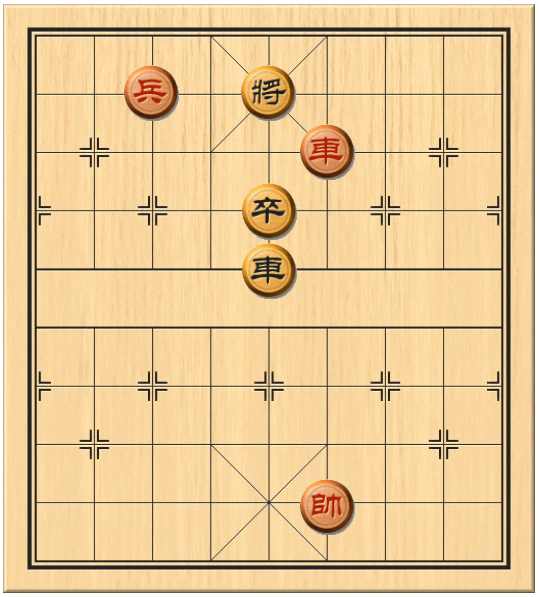
\includegraphics[width= 0.35\textwidth]{2}
		\caption{\small\textit{\color{gocco}Hình $2$.}}
		\vspace*{-10pt}
	\end{figure}
	$2.$ Hình $2$, bên Đen dường như đang nắm lợi thế lớn vì còn song Xe và đơn Chốt áp sát, chỉ cần ép Đỏ đấu xe là có thể giành thắng lợi bất cứ lúc nào. Nhưng Đỏ được quyền đi trước và không dễ để điều đó xảy ra, Đỏ đi:
	\vskip 0.05cm
	$\pmb{1)}$ P$7-5$ T$5/7$\quad  $\pmb{2)}$ P$5/3$$(*)$ T$3.5$\quad  $\pmb{3)}$ T$5/3$$(**)$ T$5/3$\quad $\pmb{4)}$ X$2.8$ Tg$5/1$\quad $\pmb{5)}$ C$6-5$  S$4.5$ \quad$\pmb{6)}$ C$5.1$ Tg$5-4$\quad $\pmb{7)}$ C$5-6$ Tg$4-5$\quad $\pmb{8)}$ X$2-5$$(***)$ $(1-0)$.
	\vskip 0.05cm
	\textit{$(*)$ Nhờ có Tượng yểm trợ, Đỏ thoải mái bình Pháo chiếu rồi rút về chém Chốt, giải trừ mối nguy hiểm tiềm tàng. Đen chỉ biết di chuyển Tượng che chắn một cách bị động.
	\vskip 0.05cm
	$(**)$ Điều Tượng về che chắn tuyến đáy, giúp Xe dễ dàng thoát lên tham chiến, nhưng vẫn có thể dùng Pháo chiếu tướng để giữ nước tiên. Một nước đi nhẹ nhàng nhưng đầy hiệu quả.
	\vskip 0.05cm
	$(***)$ Sau khi đưa xe ra tiền tuyến, đã phối hợp chặt chẽ với Pháo – Chốt tạo ra một đợt tấn công tổng lực, bên Đen dù còn song Xe nhưng cũng đành phải cởi giáp quy hàng.}
		\begin{figure}[H]
		\vspace*{-5pt}
		\centering
		\captionsetup{labelformat= empty, justification=centering}
		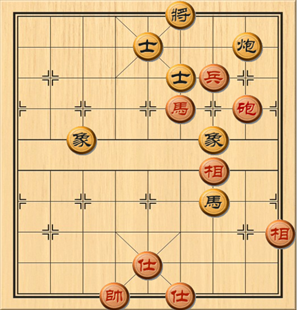
\includegraphics[width= 0.35\textwidth]{3}
		\caption{\small\textit{\color{gocco}Hình $3$.}}
		\vspace*{-10pt}
	\end{figure}
	$3.$ Hình $3$, hai bên quân lực tương tự nhau, bên Đen có hệ thống Xe -- Mã -- Chốt áp sát, chỉ cần đi X$7.2$ là có thể chiếu bí. Đỏ trong tình thế ``ngàn cân treo sợi tóc" đã xuất ra chiêu giải sát -- hoàn sát vô cùng cao tay. Đỏ đi:
	\vskip 0.05cm
	$\pmb{1)}$ T$5.3$$(*)$ X$7/2$\quad $\pmb{2)}$ P$3.3$ X$7/5$\quad $\pmb{3)}$ X$7.3$ Tg $4.1$\quad $\pmb{4)}$ C$5.1$$(**)$ S$6.5$\quad $\pmb{5)}$ X$7-3$$(***)$ $(1-0)$.
	\vskip 0.05cm
	\textit{$(*)$ Đỏ treo Tượng để dùng Pháo bắt xe, một nước đi quá đỗi bất ngờ và ảo diệu, vừa tránh nước X$7.2$ sát cục của Đen, vừa mở rộng mặt Tướng tạo thế công trong tương lai.
	\vskip 0.05cm
	$(**)$ Dùng Chốt đánh thẳng vào cửu cung, nước đi vô cùng dứt khoát, Tướng không thể ăn vào vì lộ mặt, lại một lần nữa chúng ta thấy được sự tinh tế và sâu sắc của nước treo Tượng trước đó.
	\vskip 0.05cm
	$(***)$ Đen chỉ có thể dùng Sĩ ăn lên Chốt, tạo cơ hội cho Xe Đỏ ra tay hành động. Đen mất xe, chắc chắn thua cuộc.}
	\vskip 0.05cm
\hfill \textit{Xem tiếp trang $57$.}
%	\textbf{\textit{\color{gocco}Câu đố kỳ này:}}
%	Đỏ sẽ tận dụng nước tiên và vận dụng những nước đi của Tượng như thế nào để giành chiến thắng trong các hình cờ dưới đây?
%	\begin{figure}[H]
%		\vspace*{-5pt}
%		\centering
%		\captionsetup{labelformat= empty, justification=centering}
%		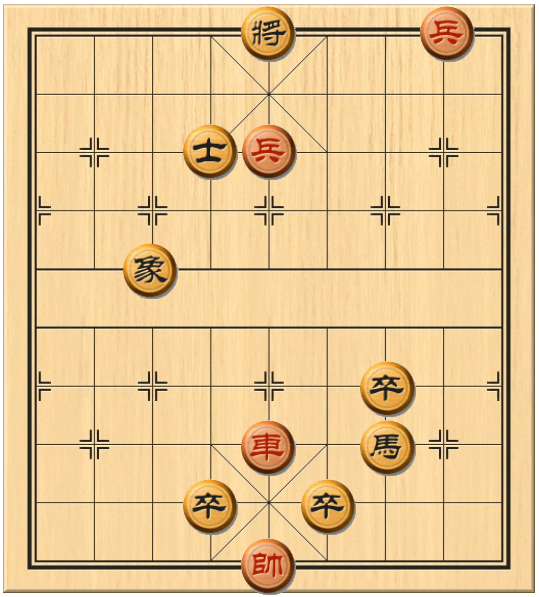
\includegraphics[width= 0.35\textwidth]{4}
%		\caption{\small\textit{\color{gocco}Hình $4$.}}
%		\vspace*{-10pt}
%	\end{figure}
%	\textit{Đáp án tham khảo}: $\pmb{1)}$ P$9-5$ T$5/3$\quad $\pmb{2)}$ P$5/5$ T$3.5$\quad $\pmb{3)}$ T$5.7$ T$5.3$ \quad$\pmb{4)}$ T$3.5$ T$3/5$\quad $\pmb{5)}$ T$5.3$ T$5.7$\quad $\pmb{6)}$ P$2-5$ $(1-0)$
%	\begin{figure}[H]
%		\vspace*{5pt}
%		\centering
%		\captionsetup{labelformat= empty, justification=centering}
%		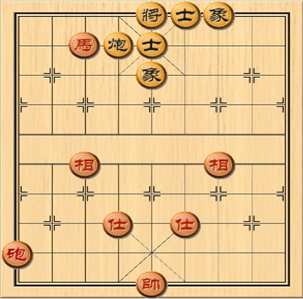
\includegraphics[width= 0.35\textwidth]{5}
%		\caption{\small\textit{\color{gocco}Hình $5$.}}
%		\vspace*{-10pt}
%	\end{figure}
%%	
%%	\vspace*{50pt}
%%	\vfill\null
%%
%%	\vskip 0.05cm
%	\textit{Đáp án tham khảo}: $\pmb{1)}$ C$7-6$ T$5.7$\quad  $\pmb{2)}$ T$9.7$ T$7/9$\quad $\pmb{3)}$ T$7/5$ T$9.7$\quad $\pmb{4)}$ Tg$4-5$ T$7/5$\quad $\pmb{5)}$ Tg$5-6$ S$6/5$\quad $\pmb{6)}$ C$6-5$ $(1-0)$
%	\vskip 0.05cm   
%	\textit{Chú thích}: C: Chốt (Tốt), X: Xe, M: Mã, P: Pháo, Tg: Tướng, S: Sĩ, T: Tượng.
\end{multicols}





